\documentclass[UTF8,a4paper,12pt]{ctexart}
\usepackage{geometry}
\usepackage{graphicx}
\usepackage{booktabs}
\usepackage{longtable}
\usepackage{array}
\usepackage{float}
\usepackage{hyperref}
\usepackage{xcolor}
\usepackage{listings}
\usepackage{amsmath}
\usepackage{caption}
\usepackage{subcaption}
\usepackage{setspace}
\usepackage{url}

\geometry{left=2.6cm,right=2.6cm,top=2.5cm,bottom=2.5cm}
\onehalfspacing
\hypersetup{colorlinks=true,linkcolor=blue,urlcolor=blue}
\setlength{\parindent}{2em}
\setlength{\parskip}{0.25em}
\captionsetup{font=small,labelfont=normalfont,textfont=normalfont}
\setlength{\intextsep}{8pt plus 2pt minus 2pt}
\setlength{\textfloatsep}{10pt plus 2pt minus 2pt}
\setlength{\floatsep}{8pt plus 2pt minus 2pt}

\lstset{
  basicstyle=\ttfamily\small,
  breaklines=true,
  frame=single,
  columns=fullflexible,
  keywordstyle=\color{blue},
  commentstyle=\color{gray},
  stringstyle=\color{teal},
  showstringspaces=false
}

\newcommand{\code}[1]{\texttt{#1}}

\begin{document}

\begin{titlepage}
\centering
\vspace*{2.2cm}
{\zihao{1}\bfseries 传感器与检测技术实验报告\par}
\vspace{1.2cm}
{\zihao{2}\bfseries 实验四：MPU6050/MPU6500 惯性传感器驱动、标定与误差分析\par}
\vspace{2.2cm}
\begin{tabular}{rl}
课程名称：& 传感器与检测技术\\[0.6cm]
指导手册：& 实验四指导手册 MPU6050标定版\\[0.6cm]
实验对象：& ESP32-S3 + MPU6500 惯性传感器模块\\[0.6cm]
开发方式：& ESP-IDF + Python 数据后处理\\[0.6cm]
姓名：& 罗丹\\[0.6cm]
学号：& 2251801014\\[0.6cm]
GitHub：& \url{https://github.com/gf-be/ESP32_course}\\[0.6cm]
日期：& \today\\
\end{tabular}
\vfill
{\zihao{4}福建理工大学\par}
\end{titlepage}

\tableofcontents
\clearpage

\section{实验目的与软件代仪器思路}
本实验按照《实验四指导手册 MPU6050标定版》完成惯性传感器的底层驱动、误差体验、六位置加速度计标定、陀螺仪温度补偿、Allan 方差噪声分析和互补滤波姿态估计。实验的核心目标不是简单读取 IMU 原始数据，而是理解同一颗 MEMS 传感器在标定前后精度差异，以及工业 IMU 产品为什么需要复杂的出厂标定流程。

指导手册以 MPU6050 为例。本实验实际模块读取到的身份寄存器为 \code{WHO\_AM\_I = 0x70}，对应 MPU6500 或兼容模块。MPU6050 与 MPU6500 在本实验使用的 I2C 地址、加速度计寄存器、陀螺仪寄存器和主要配置寄存器上兼容，因此本实验沿用指导手册的 MPU60x0 寄存器体系；同时根据 MPU6500 数据手册修正温度换算公式。该差异已经在代码和报告中说明，不影响实验原理。

本实验还体现了指导手册提出的“软件代仪器”思想。加速度计标定使用地球重力作为 1 g 绝对基准，不依赖精密转台；陀螺仪温度补偿使用冰箱、冰袋和自然回温过程近似替代温箱；Allan 方差使用 1 小时静置数据和 Python 计算替代专用 MEMS 噪声分析仪；动态误差观察使用轻弹桌面、手机振动和手动旋转替代振动台与速率转台。通过这些替代方法，可以在普通课程实验条件下完成接近工业标定流程的核心训练。

\begin{table}[H]
\centering
\caption{指导手册报告要求与本报告对应位置}
\begin{tabular}{p{0.38\textwidth}p{0.24\textwidth}p{0.26\textwidth}}
\toprule
报告要求 & 对应章节 & 完成情况\\
\midrule
实验目的 + 软件代仪器思路 & 第 1 节 & 已完成\\
MPU6050 初始化参数选择理由 & 第 3 节 & 已完成，并说明 MPU6500 兼容调整\\
六位置标定：过程、Python 输出、精度对比 & 第 5 节 & 已完成\\
温度补偿：冰箱实验、曲线图、残差统计 & 第 6 节 & 已完成\\
Allan 方差：曲线、ARW/BI、datasheet 对比 & 第 7 节 & 已完成\\
互补滤波姿态实验 & 第 8 节 & 已完成\\
思考题 & 第 10 节 & 5 题均作答\\
AI 协作记录与实验总结 & 第 11、12 节 & 已完成\\
\bottomrule
\end{tabular}
\end{table}

\section{实验硬件与软件环境}
\subsection{硬件环境}
本实验使用 ESP32-S3 作为主控，惯性传感器模块为实际识别到的 MPU6500。虽然指导手册示例使用 ESP32-DevKitC 与 MPU6050，实际实验中使用的 ESP32-S3 可通过修改 I2C 引脚完成相同功能。硬件环境如表 \ref{tab:hardware} 所示。

\begin{table}[H]
\centering
\caption{实验硬件环境}
\label{tab:hardware}
\begin{tabular}{lll}
\toprule
设备 & 实际配置 & 用途\\
\midrule
主控板 & ESP32-S3 & I2C 读取 IMU、串口输出、姿态计算\\
IMU 模块 & MPU6500 兼容模块 & 三轴加速度、三轴陀螺仪、温度测量\\
辅助固定件 & 方正铁盒/稳定支撑面 & 六位置标定时固定姿态\\
低温环境 & 冰箱、冰袋 & 陀螺仪温度补偿实验\\
电脑 & Windows & ESP-IDF 编译、串口记录、Python 分析\\
\bottomrule
\end{tabular}
\end{table}

\subsection{接线方式}
实际接线与手册示例略有差异。ESP32-S3 使用 GPIO21 作为 SDA，GPIO8 作为 SCL。该变化只影响代码中的 I2C 引脚定义，不影响 I2C 读写流程。

\begin{table}[H]
\centering
\caption{MPU6500 与 ESP32-S3 实际接线}
\begin{tabular}{lll}
\toprule
IMU 引脚 & ESP32-S3 引脚 & 说明\\
\midrule
VCC & 3.3V & 模块供电\\
GND & GND & 共地\\
SDA & GPIO21 & I2C 数据线\\
SCL & GPIO8 & I2C 时钟线\\
AD0 & GND & I2C 地址 0x68\\
\bottomrule
\end{tabular}
\end{table}

\subsection{软件环境}
固件采用 ESP-IDF 编写，数据分析使用 Python。提交包保留了 ESP32 工程代码、关键 CSV 数据和图表文件，便于复查实验结论。

\begin{table}[H]
\centering
\caption{实验软件环境}
\begin{tabular}{ll}
\toprule
软件或库 & 用途\\
\midrule
ESP-IDF & ESP32-S3 固件开发\\
Python & 串口记录、数据分析和绘图\\
NumPy / pandas & CSV 读取、均值统计和矩阵计算\\
matplotlib & 标定、温度、Allan 和姿态图绘制\\
Allan 方差分析脚本 & 计算 ADEV、ARW 和 BI\\
\bottomrule
\end{tabular}
\end{table}

\section{MPU6050/MPU6500 初始化参数选择}
\subsection{身份识别与兼容性处理}
固件启动后首先读取 \code{WHO\_AM\_I} 寄存器。本实验新模块返回 \code{0x70}，因此按 MPU6500 处理；如果返回 \code{0x68}，则可按 MPU6050 处理。两者在本实验所需的 \code{PWR\_MGMT\_1}、\code{CONFIG}、\code{SMPLRT\_DIV}、\code{GYRO\_CONFIG}、\code{ACCEL\_CONFIG} 和数据输出寄存器上兼容。

\begin{lstlisting}[language=C]
#define MPU6050_ID       0x68
#define MPU6500_ID       0x70
#define MPU_ADDR         0x68

err = mpu_read_byte(REG_WHO_AM_I, &who);
if (who != MPU6050_ID && who != MPU6500_ID) {
    return ESP_ERR_NOT_FOUND;
}
mpu_who_am_i = who;
\end{lstlisting}

\subsection{采样率、DLPF 与量程选择}
本实验的重点是静态标定、温漂观察和低速姿态估计，因此选择较高分辨率而非最大动态范围。采样周期约为 5 ms，对应 200 Hz 输出，满足手册中连续读取、Allan 方差和互补滤波的需求。DLPF 设置为 \code{CONFIG=0x03}，约 44 Hz 截止，可抑制高频振动和电噪声。加速度计设置为 \(\pm 2g\)，提高六位置静态标定分辨率；陀螺仪设置为 \(\pm 250^\circ/s\)，提高零偏和温漂测量灵敏度。

\begin{table}[H]
\centering
\caption{MPU 初始化参数}
\begin{tabular}{lll}
\toprule
寄存器或参数 & 实际设置 & 选择理由\\
\midrule
\code{WHO\_AM\_I} & \code{0x70} & 实际模块为 MPU6500\\
\code{PWR\_MGMT\_1} & \code{0x00} & 清除睡眠位，唤醒传感器\\
\code{CONFIG} & \code{0x03} & DLPF 约 44 Hz，抑制高频噪声\\
\code{SMPLRT\_DIV} & \code{4} & 配合任务周期约 200 Hz 输出\\
\code{ACCEL\_CONFIG} & \code{0x00} & \(\pm 2g\)，提高静态标定分辨率\\
\code{GYRO\_CONFIG} & \code{0x00} & \(\pm 250^\circ/s\)，提高零偏测量灵敏度\\
\bottomrule
\end{tabular}
\end{table}

MPU6500 与 MPU6050 的温度公式不同。代码中根据 \code{WHO\_AM\_I} 自动选择温度换算公式，避免把 MPU6500 的温度读数按 MPU6050 公式错误换算。

\begin{lstlisting}[language=C]
static float temp_c_from_raw(int16_t raw) {
    if (mpu_who_am_i == MPU6500_ID) {
        return (float)raw / 333.87f + 21.0f;
    }
    return (float)raw / 340.0f + 36.53f;
}
\end{lstlisting}

\section{基础读取与动态误差体验}
\subsection{I2C 读取与数据输出}
固件能够稳定输出加速度、陀螺仪和温度数据。输出格式如下：

\begin{lstlisting}
CSV,t,ax_g,ay_g,az_g,gx_dps,gy_dps,gz_dps,temp_c
\end{lstlisting}

更换新模块后，8 秒检查数据共 304 行，其中 304 行都有非零陀螺仪输出。静止均值约为 gx = 0.630 deg/s、gy = 1.056 deg/s、gz = -0.178 deg/s，说明新模块陀螺仪输出正常，可以用于后续温度补偿、Allan 方差和姿态估计。

\subsection{振动与旋转观察}
动态误差体验按照手册 Step 3 的思路进行。静止基线文件为 \code{vibration\_baseline\_static.csv}，静止时加速度模长标准差为 0.002393 g。轻弹桌面时 \(|a|\) 标准差增大到 0.049189 g，约为静止基线的 20.56 倍；手机振动时 \(|a|\) 标准差为 0.009407 g，约为静止基线的 3.93 倍。说明加速度计对外部振动非常敏感，实际姿态融合不能直接完全信任加速度瞬时值。

\begin{figure}[H]
\centering
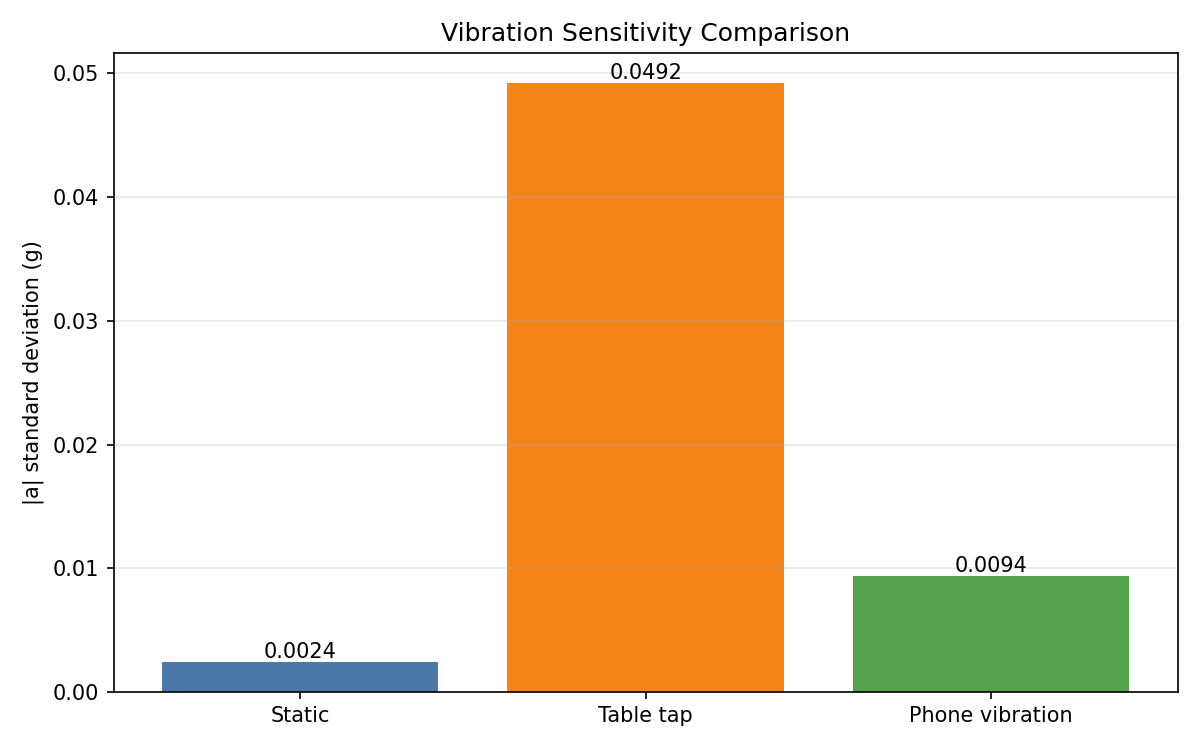
\includegraphics[width=0.82\textwidth,height=0.45\textheight,keepaspectratio]{assets/fig_vibration_norm_std.png}
\caption{静止、轻弹桌面和手机振动下的加速度模长标准差对比}
\end{figure}

手动旋转实验使用 \code{rotation\_observation\_rerun.csv}。重做数据中加速度投影在三个轴之间明显变化，gz 最大值约为 71.977 deg/s，说明传感器姿态发生了实质性改变。

\begin{figure}[H]
\centering
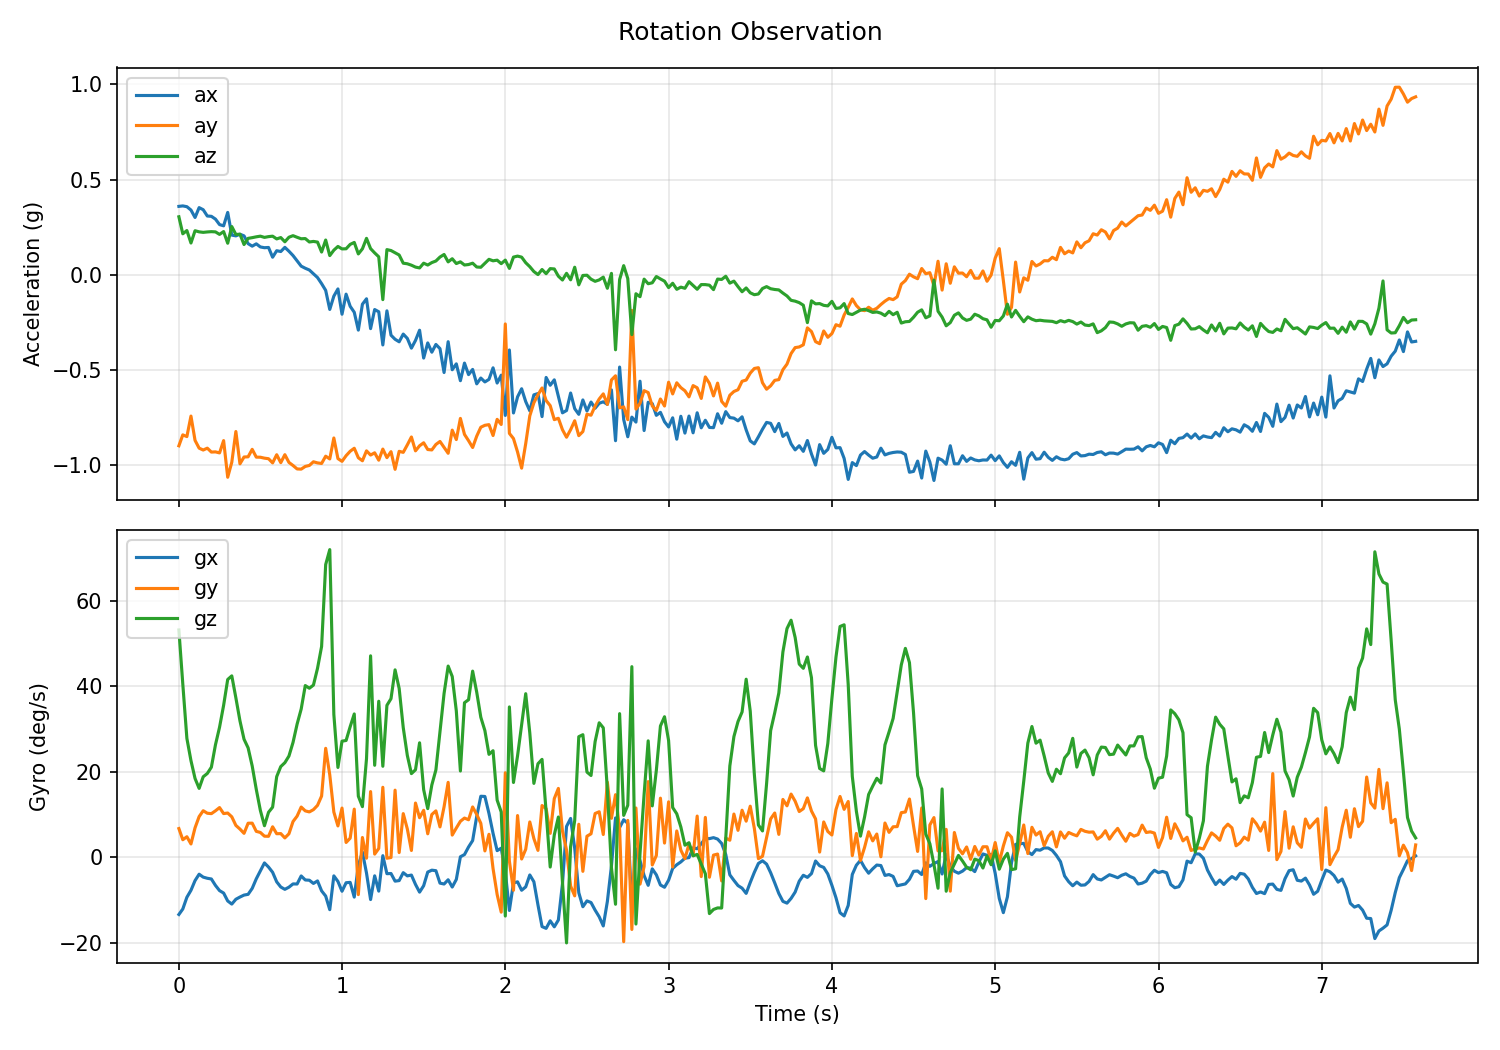
\includegraphics[width=0.88\textwidth,height=0.48\textheight,keepaspectratio]{assets/fig_rotation_observation.png}
\caption{手动旋转时加速度与陀螺仪输出变化}
\end{figure}

\section{六位置加速度计标定}
\subsection{标定模型}
六位置标定使用地球重力作为绝对 1 g 基准。对每个静止姿态采集 1200 行数据并取均值，用线性模型拟合：

\begin{equation}
\mathbf{a}_{meas}=A\mathbf{a}_{true}+\mathbf{c}
\end{equation}

其中 \(A\) 表示比例因子、轴间耦合和非正交误差综合矩阵，\(\mathbf{c}\) 表示零偏。运行时补偿公式为：

\begin{equation}
\mathbf{a}_{corrected}=A^{-1}(\mathbf{a}_{meas}-\mathbf{c})
\end{equation}

实验初期曾使用手机水平仪辅助找平，但手机背面摄像头凸起会带来约 3 deg 的放置误差。最终改用较方正的铁盒固定模块，并统一六面采样流程。

\subsection{六位置数据}
\begin{table}[H]
\centering
\caption{最终六位置加速度计均值}
\small
\begin{tabular}{lrrrrr}
\toprule
位置 & 方向 & ax & ay & az & \(|a|\)\\
\midrule
P1 & +X & 1.003491 & 0.011601 & 0.065739 & 1.005709\\
P2 & -X & -0.995915 & 0.000845 & -0.039087 & 0.996682\\
P3 & -Y & 0.007937 & -0.990993 & -0.054641 & 0.992530\\
P4 & +Y & -0.000461 & 1.003540 & 0.081213 & 1.006821\\
P5 & -Z & 0.058814 & 0.079489 & -1.002104 & 1.006970\\
P6 & +Z & -0.051288 & -0.066962 & 1.028665 & 1.032117\\
\bottomrule
\end{tabular}
\end{table}

\subsection{Python 输出与标定参数}
最小二乘拟合得到：

\begin{lstlisting}
A =
[[ 0.99970322 -0.00419880 -0.05505064]
 [ 0.00537800  0.99726690 -0.07322512]
 [ 0.05241328  0.06792680  1.01538444]]

c = [0.00376301, 0.00625345, 0.01329749]

Mean before: 10.401 mg
Mean after: 0.021 mg
Improvement ratio: 497.17x
\end{lstlisting}

写入 ESP32 的运行时补偿参数如下：

\begin{lstlisting}[language=C]
static const float ACCEL_A_INV[3][3] = {
    {0.99745688f, 0.00051362f, 0.05411571f},
    {-0.00911479f, 0.99783450f, 0.07146532f},
    {-0.05087812f, -0.06677926f, 0.97727439f},
};
static const float ACCEL_C_BIAS[3] = {
    0.00376301f, 0.00625345f, 0.01329749f
};
\end{lstlisting}

\subsection{标定效果}
\begin{table}[H]
\centering
\caption{六位置标定前后模长误差对比}
\begin{tabular}{lrr}
\toprule
位置 & 标定前误差 & 标定后误差\\
\midrule
P1 & 5.709 mg & 0.026 mg\\
P2 & 3.318 mg & 0.026 mg\\
P3 & 7.470 mg & 0.019 mg\\
P4 & 6.821 mg & 0.019 mg\\
P5 & 6.970 mg & 0.017 mg\\
P6 & 32.117 mg & 0.017 mg\\
平均 & 10.401 mg & 0.021 mg\\
\bottomrule
\end{tabular}
\end{table}

\begin{figure}[H]
\centering
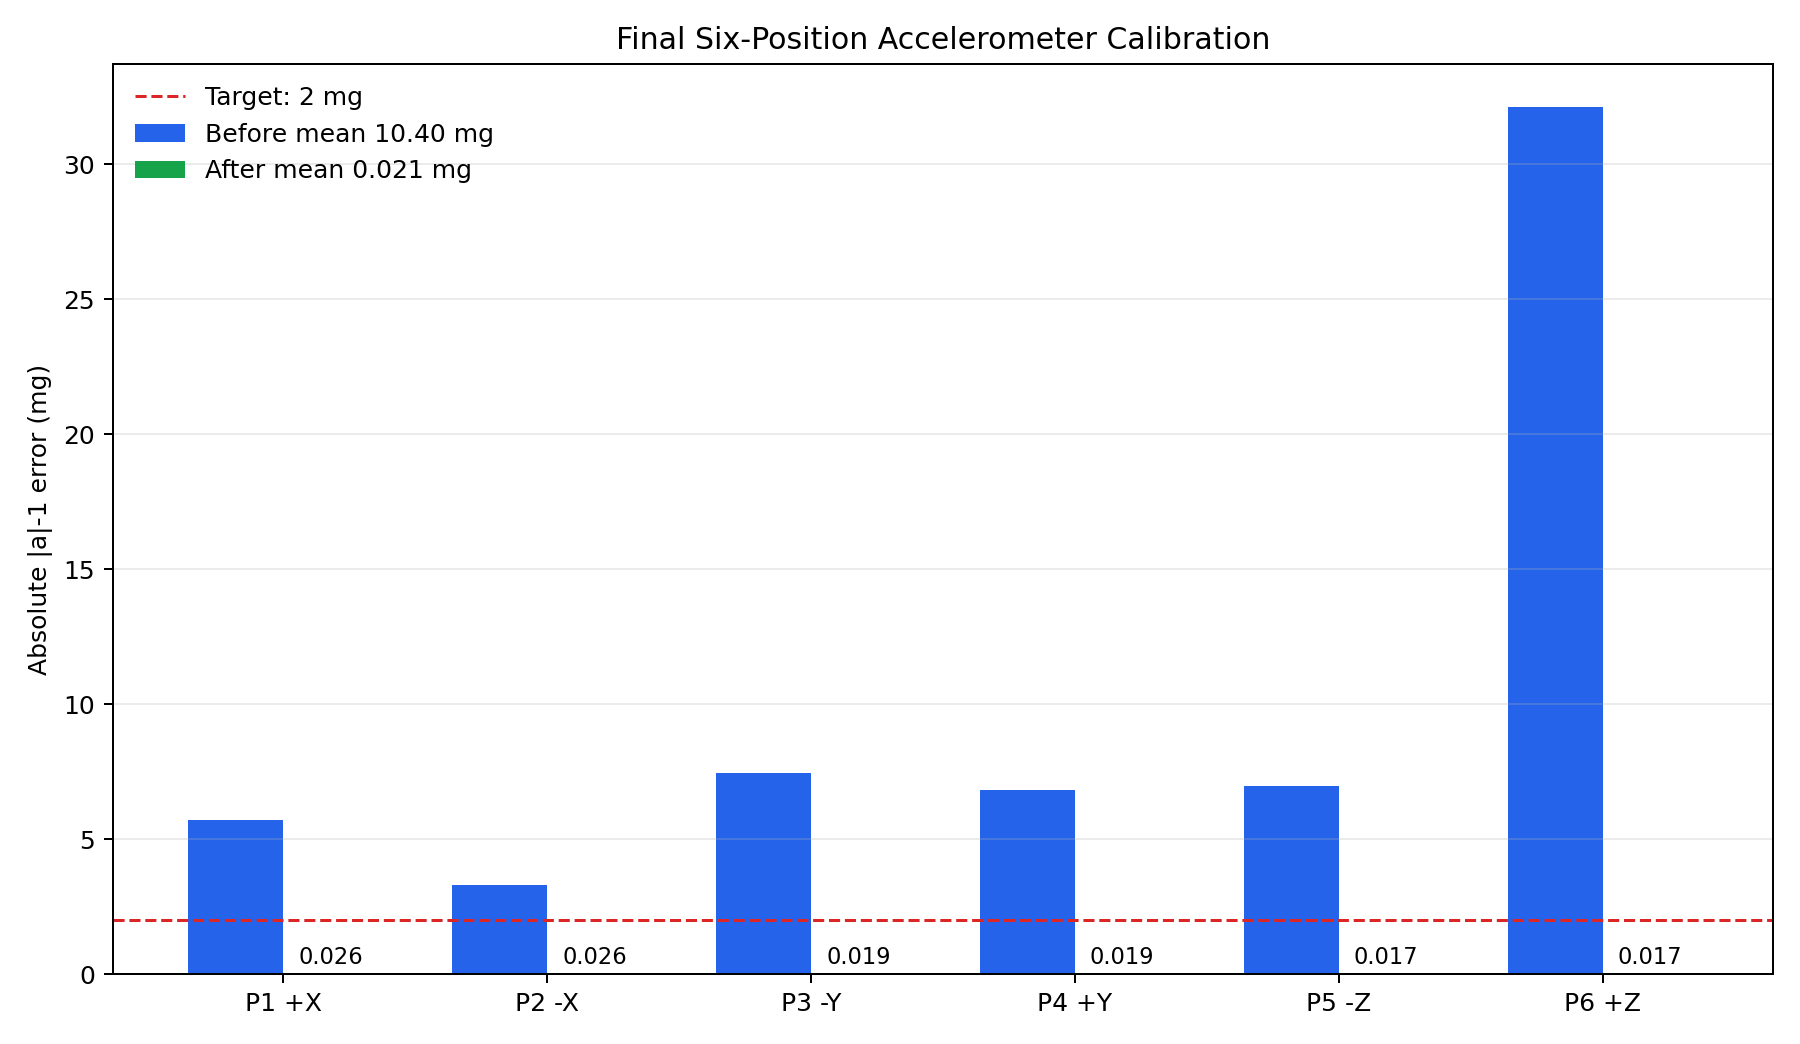
\includegraphics[width=0.84\textwidth,height=0.45\textheight,keepaspectratio]{assets/fig_accel_final_group_calibration_errors.png}
\caption{六位置标定前后误差对比}
\end{figure}

手册要求标定后误差小于 5 mg，本实验最终平均模长误差为 0.021 mg，最大模长误差为 0.026 mg，明显满足验收要求。

\section{陀螺仪温度补偿}
\subsection{温度实验过程}
指导手册建议使用冰箱冷藏到低温后自然回温。本实验最初直接冷藏后的 \code{gyro\_warmup\_after\_fridge\_600s.csv} 温度范围只有 24.98--26.79 degC，未形成有效温度扫描，因此只作为近室温漂移观察。随后使用冰袋靠近 MPU6500 进行降温，再让模块自然回温，最终数据文件为 \code{gyro\_icepack\_cooling\_warmup\_600s.csv}。

完整数据共 23985 行，温度范围为 13.09--22.02 degC。由于移动冰袋时可能带来轻微机械扰动，分析时按以下条件筛选静止点：

\begin{lstlisting}
0.98 <= |a| <= 1.04
abs(gx), abs(gy), abs(gz) < 2.5 deg/s
\end{lstlisting}

过滤后保留 23964 行，剔除 21 行扰动数据。

\subsection{二次多项式拟合}
按指导手册建议，以 0.5 degC 为温度分箱取中值，再对每个陀螺仪轴拟合二次多项式：

\begin{equation}
b(T)=c_0+c_1T+c_2T^2
\end{equation}

\begin{table}[H]
\centering
\caption{陀螺仪温度补偿拟合结果}
\small
\begin{tabular}{lrrrr}
\toprule
轴 & \(c_0\) & \(c_1\) & \(c_2\) & 残差标准差\\
\midrule
gx & 0.7319705145 & 0.0022361197 & -0.0003042901 & 0.009083 deg/s\\
gy & 1.0369519387 & 0.0122930857 & -0.0004033613 & 0.003572 deg/s\\
gz & -0.4898115878 & 0.0153560372 & -0.0000176913 & 0.006992 deg/s\\
\bottomrule
\end{tabular}
\end{table}

\begin{figure}[H]
\centering
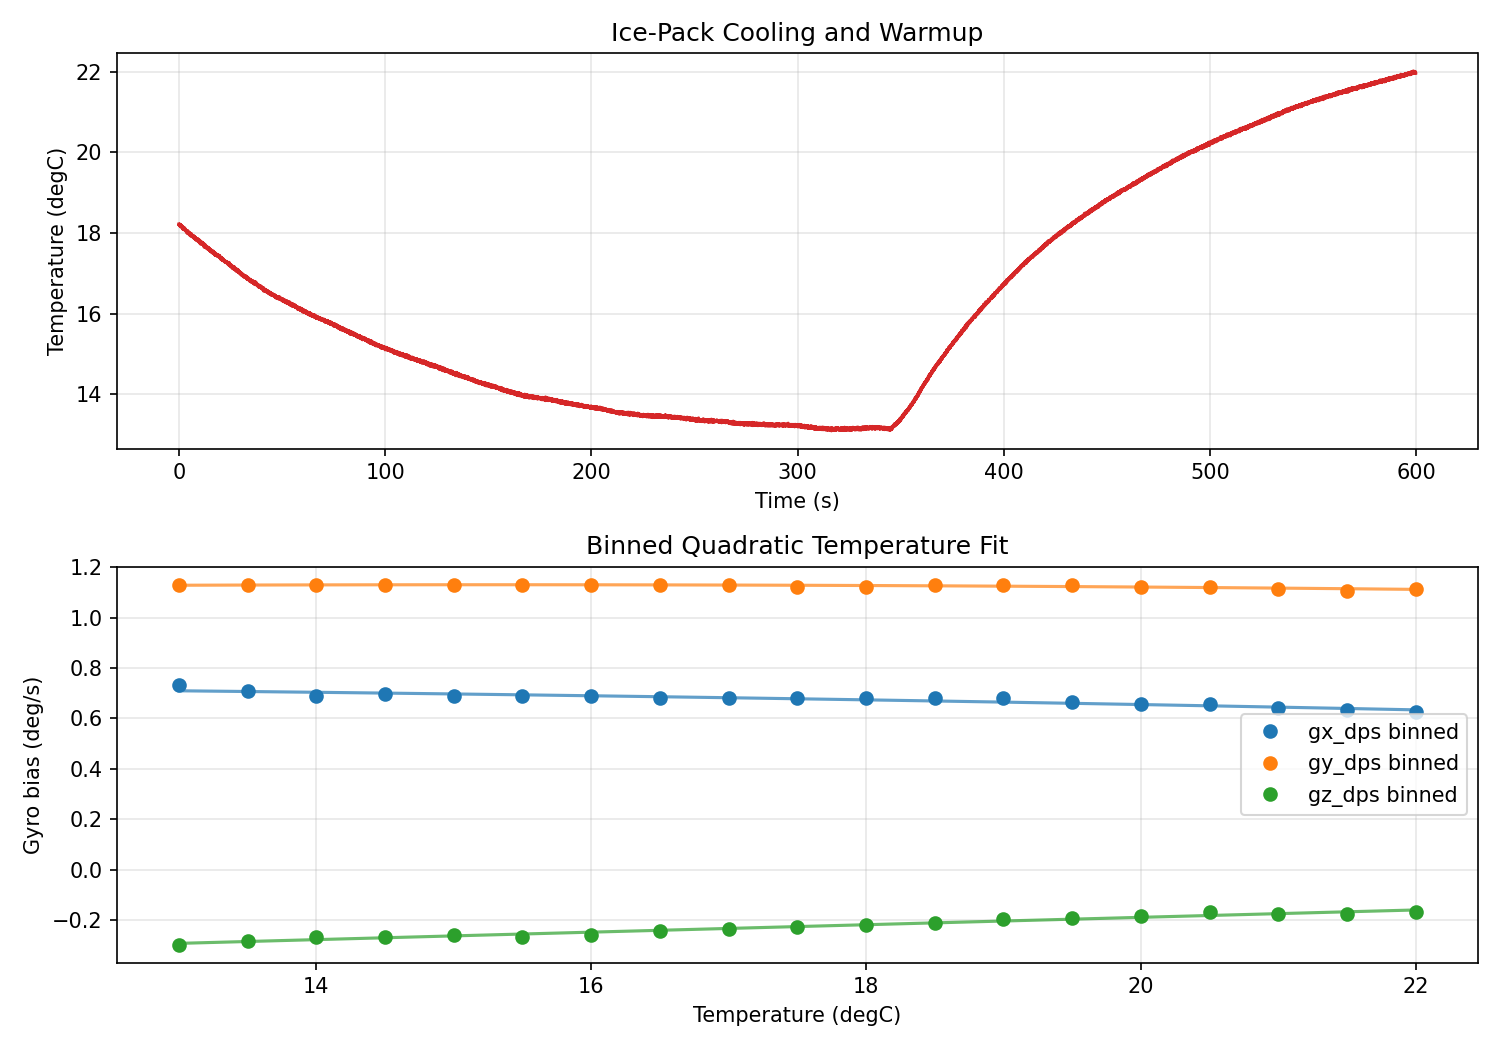
\includegraphics[width=0.86\textwidth,height=0.48\textheight,keepaspectratio]{assets/fig_temperature_icepack_fit.png}
\caption{冰袋降温回温过程与陀螺仪温度补偿拟合曲线}
\end{figure}

三轴分箱拟合残差均小于 0.05 deg/s，满足指导手册对残差的验收要求。需要说明的是，本实验最低温度为 13.09 degC，未达到手册建议的 10 degC 以下，因此温度补偿模型更适合解释 13--22 degC 有限温区内的漂移规律。

\section{Allan 方差实测}
\subsection{数据采集}
Allan 方差数据文件为 \code{allan\_raw\_1h.csv}，静止采集 719946 行，传感器时间长度为 3599.725 s，约 60 min。平均采样率为 200.000 Hz，分析轴为 \code{gz\_dps}。采集期间模块保持静止，用于估计该传感器在静态条件下的真实噪声底。

\subsection{分析结果}
\begin{table}[H]
\centering
\caption{Allan 方差主要结果}
\begin{tabular}{lr}
\toprule
指标 & 数值\\
\midrule
ARW at tau=1s & 0.005880 deg/s\\
ARW & 0.045544 deg/sqrt(min)\\
ARW & 0.352780 deg/sqrt(hr)\\
BI & 0.001145 deg/s at tau=899.929 s\\
\bottomrule
\end{tabular}
\end{table}

\begin{figure}[H]
\centering
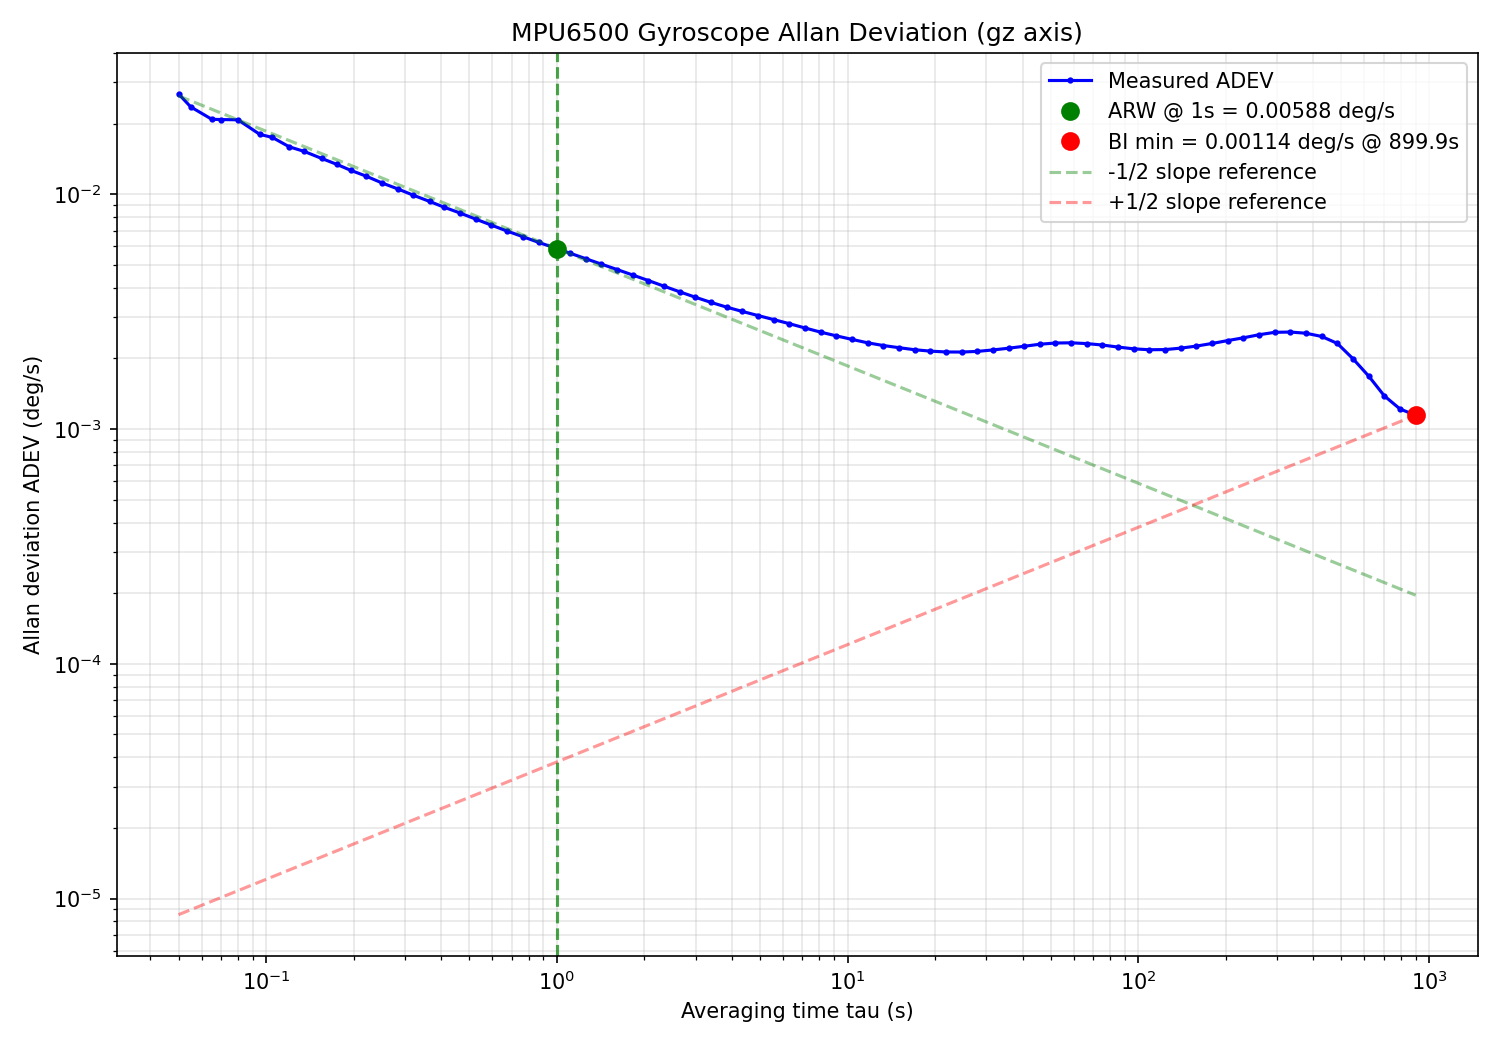
\includegraphics[width=0.86\textwidth,height=0.48\textheight,keepaspectratio]{assets/fig_allan_curve_gz.png}
\caption{MPU6500 gz 轴 Allan 方差曲线}
\end{figure}

\subsection{与 datasheet 对比}
指导手册给出的 MPU6050 陀螺仪噪声密度典型值约为 0.005 deg/s/sqrt(Hz)。手册示例中典型 ARW 约为 0.08--0.15 deg/sqrt(s)，即约 4.8--9.0 deg/sqrt(hr)。本实验实测 gz 轴 ARW 为 0.005880 deg/s at tau=1s，折算为 0.352780 deg/sqrt(hr)。该结果低于手册典型范围，可能与实际器件为 MPU6500、新模块状态较好、分析轴为较稳定的 gz 轴、采样过程较稳定有关。由于不同资料对 ARW 单位换算口径不同，本报告同时列出 tau=1s ADEV、deg/sqrt(min) 和 deg/sqrt(hr)，保证结果可复算。

1 小时数据可以较可靠读出 ARW 和 BI 的量级，但对更大 tau 处的速率随机游走和长期温漂不够充分。若要完整观察曲线末端上翘段，需要更长时间的静置数据和更稳定的时间基准。

\section{互补滤波姿态估计}
\subsection{滤波原理}
加速度计长期可以给出重力方向，但会受到振动和线加速度影响；陀螺仪短期响应快，但积分后会漂移。互补滤波将两者结合：

\begin{align}
roll &= 0.98\cdot roll_{gyro}+0.02\cdot roll_{acc}\\
pitch &= 0.98\cdot pitch_{gyro}+0.02\cdot pitch_{acc}
\end{align}

固件输出格式为：

\begin{lstlisting}
ATT,t,roll_deg,pitch_deg,roll_acc_deg,pitch_acc_deg,gx_dps,gy_dps,temp_c
\end{lstlisting}

\subsection{连续姿态实验}
单独打开串口采集时发现 ESP32 可能复位。如果复位时传感器已经处于倾斜状态，固件启动 2 秒自动归零会把该倾斜状态作为新零点。因此最终采用连续记录 \code{attitude\_continuous\_sequence.csv}，避免反复打开串口造成复位。

\begin{table}[H]
\centering
\caption{互补滤波姿态实验结果}
\begin{tabular}{lrrl}
\toprule
片段 & roll 均值 & pitch 均值 & 说明\\
\midrule
初始水平 & -0.043 deg & 0.004 deg & 水平零点稳定\\
倾斜 A & 152.204 deg & 42.143 deg & pitch 明显响应\\
回到水平 & -1.352 deg & 0.016 deg & 基本回零\\
倾斜 B & 56.851 deg & 42.725 deg & 第二组倾斜稳定\\
\bottomrule
\end{tabular}
\end{table}

\begin{figure}[H]
\centering
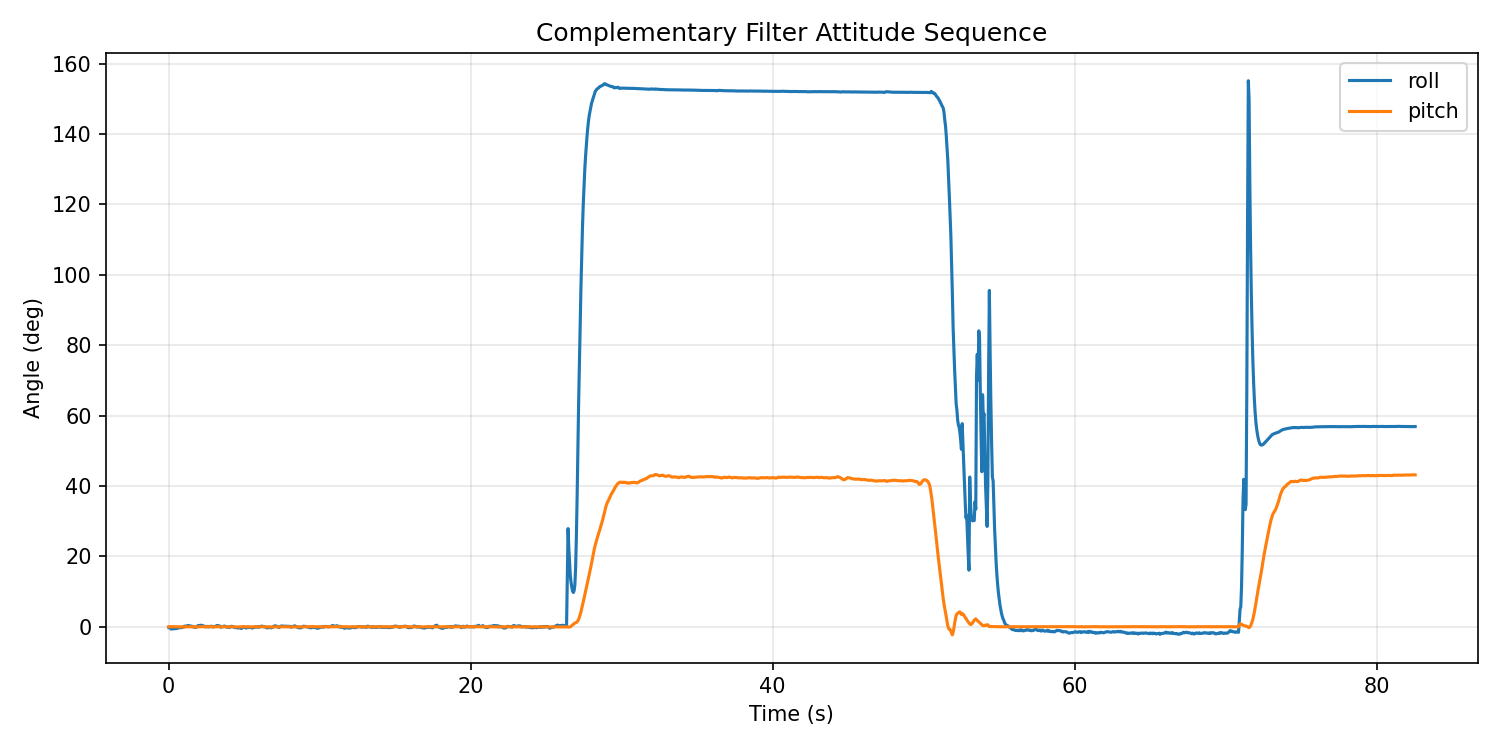
\includegraphics[width=0.86\textwidth,height=0.48\textheight,keepaspectratio]{assets/fig_attitude_sequence.png}
\caption{连续倾斜序列中的 roll/pitch 输出}
\end{figure}

早期晃动数据中出现过角度边界跳变，之后固件加入角度环绕修正，将相对加速度角限制到 [-180 deg, 180 deg]。修正后的晃动返回数据表明姿态没有发散，回到水平后 pitch 约为 -0.1 deg，roll 有 2--3 deg 残余偏差，但整体稳定。

\begin{figure}[H]
\centering
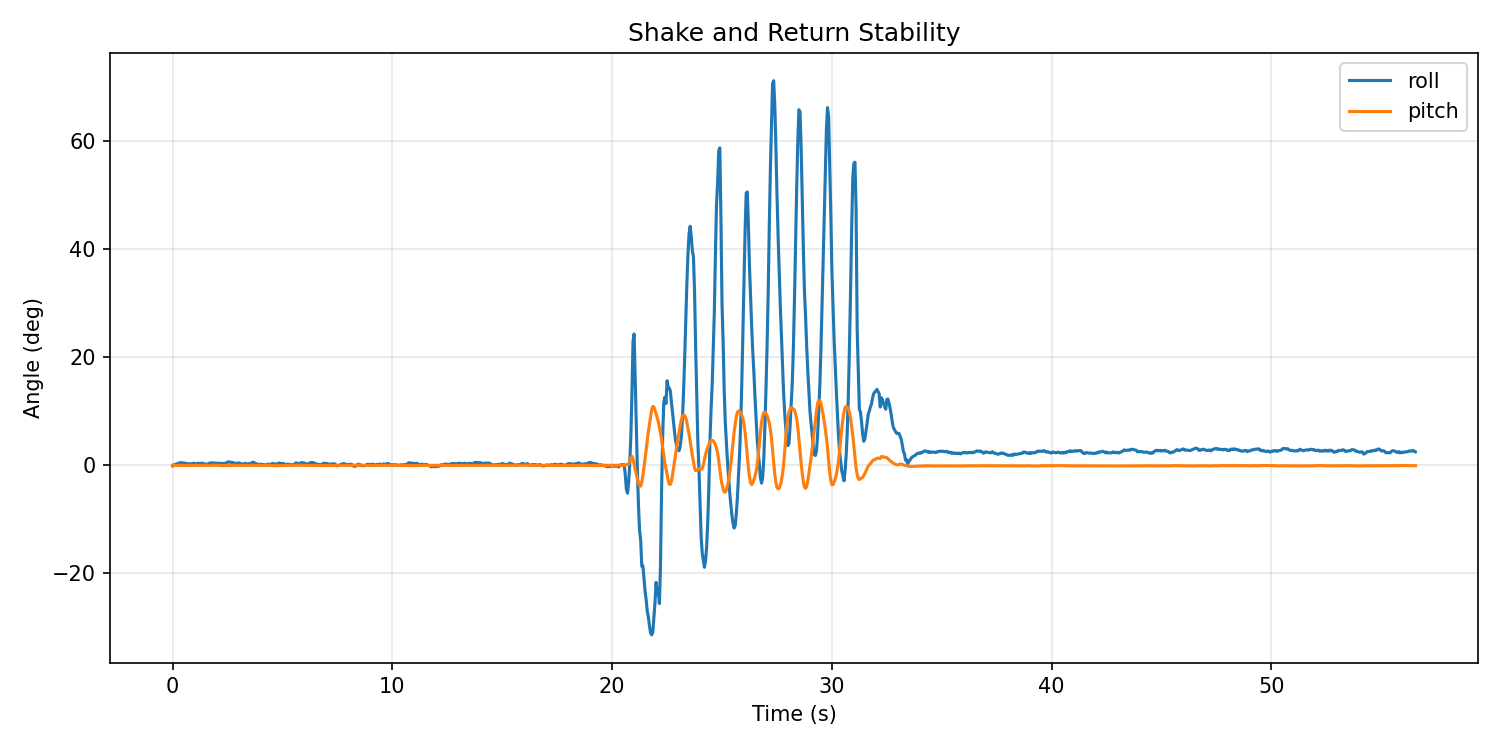
\includegraphics[width=0.86\textwidth,height=0.48\textheight,keepaspectratio]{assets/fig_attitude_shake_return.png}
\caption{晃动后返回水平的姿态稳定性}
\end{figure}

\section{实验结果汇总}
\begin{table}[H]
\centering
\caption{实验结果汇总}
\begin{tabular}{p{0.26\textwidth}p{0.18\textwidth}p{0.44\textwidth}}
\toprule
实验项目 & 完成情况 & 主要结果\\
\midrule
I2C 读取与身份识别 & 完成 & 新模块 \code{WHO\_AM\_I = 0x70}\\
连续 IMU 数据读取 & 完成 & 稳定输出加速度、陀螺仪和温度 CSV\\
动态误差观察 & 完成 & 轻弹使 \(|a|\) 标准差增至静止的 20.56 倍\\
六位置加速度标定 & 完成 & 平均模长误差 10.401 mg 降至 0.021 mg\\
温度补偿 & 完成但温区有限 & 13.09--22.02 degC，残差均小于 0.05 deg/s\\
Allan 方差 & 完成 & 1 小时、719946 行、ARW 0.352780 deg/sqrt(hr)\\
互补滤波姿态 & 完成 & 连续倾斜和晃动返回均能稳定响应\\
\bottomrule
\end{tabular}
\end{table}

\section{误差来源与改进方向}
本实验的主要误差来源包括以下几个方面。

\begin{enumerate}
\item 六位置标定对固定方式非常敏感。初期使用手机水平仪时，手机摄像头凸起带来约 3 deg 的水平误差，后续改用更稳定的铁盒固定后结果明显改善。
\item 线缆拉扯、模块贴合不平和支撑面不完全垂直会影响六位置姿态，尤其是 Z 轴两面容易出现较大的模长偏差。
\item 温度补偿实验未达到 10 degC 以下，主要原因是冷藏和冰袋降温对小模块的温差有限，同时移动冰袋容易引入机械扰动。
\item Allan 方差只采集 1 小时数据，足以估计 ARW 和 BI 量级，但不足以完整分析更长时间尺度的 RRW。
\item 姿态实验采用相对自动归零，物理安装方向与手册坐标图不完全一致，因此报告重点验证姿态响应和回零稳定性。
\end{enumerate}

后续如果继续改进，可以使用更稳定的夹具、更长时间 Allan 数据、更低温度扫描范围，以及外部 GPS 1PPS 时间基准来提升实验严谨性。

\section{思考题作答}
\subsection{为什么用 GPS 1PPS 时间基准而不用 ESP32 自带晶振？}
Allan 方差分析的横轴是集成时间 tau，tau 由采样间隔和样本数共同决定。如果采样时钟不准，曲线横轴会整体偏移，ARW、BI 等指标也会被错误读取。ESP32 自带晶振适合一般控制任务，但它会受器件误差、温度、电源和老化影响，长时间记录时 ppm 级偏差会逐渐累积。GPS 1PPS 来自卫星授时系统，长期稳定性远高于普通 MCU 晶振，用它校准或约束采样时间，可以把 Allan 方差中的“传感器噪声”与“本地时钟误差”分开。本实验未实际接入 GPS 1PPS，因此使用 ESP32 时间戳估算 200 Hz 采样率，结果足够完成课程分析；若用于工业级噪声建模，应接入 GPS 1PPS 或其他高稳定外部时钟。

\subsection{六位置标定为什么用最小二乘而不是解 6 元方程组？}
六位置标定的理论输入只有 +X、-X、+Y、-Y、+Z、-Z 六个重力方向，但实际实验并不是无噪声的 6 元方程组。每个位置都存在水平误差、夹具不平、线缆拉扯、模块贴合误差和传感器随机噪声。如果直接解方程，相当于默认六个姿态完全正确，任意一个姿态摆歪都会被硬塞进参数中，导致补偿矩阵对其他姿态反而变差。最小二乘的优点是把所有观测统一放进线性模型，在整体残差最小的意义下估计 \(A\) 和 \(c\)，对偶然误差更稳健。若每面采集更多样本或加入冗余姿态，最小二乘还可以自然吸收这些冗余信息。本实验平均模长误差由 10.401 mg 降到 0.021 mg，说明最小二乘结果显著优于未标定状态。

\subsection{冰箱实验为什么建议从冷到热？}
冰箱温度补偿实验建议从冷到热，是因为自然回温过程更容易稳定、连续、单调。传感器从低温环境取出后放在桌面不动，芯片、PCB 和空气之间逐渐达到热平衡，温度变化速度较缓，陀螺仪输出更接近“温度导致的零偏变化”。如果反过来从热到冷，通常需要持续接触冷源或反复移动位置，容易引入机械振动；同时快速降温会造成芯片内部、模块外壳和 PCB 温度不同步，甚至出现冷凝水风险，使同一温度下的零偏不唯一。反向数据不是绝对无效，但必须保证静止、降温均匀、无冷凝，并用加速度模长和陀螺阈值剔除扰动点。本实验采用冰袋降温加自然回温，并按静止条件过滤和分箱取中值。

\subsection{Allan 方差曲线在大 tau 处上翘对应什么物理过程？}
Allan 方差曲线在 tau 很大时上翘，通常对应低频漂移、速率随机游走、温度慢变化、供电漂移或环境扰动等长期过程。小 tau 区域有大量统计窗口，主要反映白噪声和角度随机游走；tau 变大后，每个窗口包含更长时间的数据，可用独立窗口数量迅速减少，估计方差会变大。以本实验 1 小时、约 720000 点数据为例，当 tau 接近几百秒甚至上千秒时，能够参与平均的窗口已经很少，曲线末端容易被一次桌面振动、室温变化或采样时钟微小漂移影响。因此 1 小时数据可以较可靠读出 ARW 和 BI 的量级，但不足以完整判断 RRW 或更长时间尺度的漂移规律。

\subsection{互补滤波的 alpha=0.98 是怎么选的？}
互补滤波的 alpha 本质上是在陀螺仪积分和加速度计倾角之间分配信任。陀螺仪短时间响应快，能跟上快速转动，但积分后会积累零偏漂移；加速度计长期能给出重力方向，适合修正低频漂移，但在振动、线加速度或手动晃动时会明显抖动。alpha=0.98 表示每次更新中约 98\% 保留陀螺仪积分，约 2\% 用加速度计慢慢拉回重力方向，是 200 Hz 姿态实验中常用的折中。若改成 0.9，加速度计权重增大，静态回零更快，但振动时姿态角会更抖；若改成 0.999，输出更平滑，但零偏修正太慢，长时间后更容易漂移。

\section{AI 协作记录}
本实验使用 AI 作为编程、数据分析和报告整理辅助工具，但硬件连接、数据采集和关键实验过程均基于实际记录完成。AI 协作主要体现在以下几个方面。

\begin{enumerate}
\item \textbf{任务拆解与检查点整理。} AI 根据《实验四指导手册 MPU6050标定版》协助将实验拆分为 I2C 读取、动态误差观察、六位置标定、温度补偿、Allan 方差和互补滤波姿态估计等任务，并帮助对照报告要求检查缺项。
\item \textbf{代码与脚本整理。} AI 协助整理 ESP32 端 IMU 读取、温度公式修正、加速度计标定补偿和互补滤波相关代码，同时辅助编写 Python 数据分析脚本，用于绘制标定、温度、Allan 和姿态图。
\item \textbf{报告排版与结果组织。} AI 协助把实测 CSV、图表、误差来源、思考题和总结整理为正式实验报告，并参考实验三的 LaTeX 报告格式生成本报告。
\item \textbf{诚信边界。} 对于没有完全达到手册理想条件的部分，例如温度未低于 10 degC、未使用 GPS 1PPS，本报告均如实说明，没有伪造实验数据或截图。
\end{enumerate}

\section{实验总结}
本实验完成了从底层 I2C 通信到 IMU 标定和姿态估计的完整流程。加速度计六位置标定后平均模长误差由 10.401 mg 降至 0.021 mg，明显优于手册要求；陀螺仪温度补偿在 13.09--22.02 degC 范围内完成二次拟合，三轴残差均小于 0.05 deg/s；Allan 方差完成约 1 小时静置实测，得到 gz 轴 ARW 和 BI；互补滤波姿态实验能够稳定响应连续倾斜，并在晃动后回到接近水平状态。

通过本实验可以直观看到：IMU 的性能不仅取决于芯片本身，也取决于标定、温度补偿、滤波和实验固定方式。未标定的 MEMS 传感器存在零偏、比例因子误差、轴间耦合和温漂；通过合理标定和数据处理，同一硬件可以获得明显更好的工程精度。实验也暴露出实际操作中的限制，例如夹具误差、温区不足、线缆拉扯和时间基准不够严格。后续若进一步提升实验质量，可以补充实物操作照片、使用更稳定夹具、扩大温度扫描范围，并接入 GPS 1PPS 进行更严格的 Allan 方差时间校准。

\appendix
\section{主要提交文件}
\begin{longtable}{p{0.36\textwidth}p{0.54\textwidth}}
\toprule
文件或目录 & 用途\\
\midrule
\code{report\_lab4\_final.tex} & 本实验 LaTeX 报告源文件\\
\code{report\_lab4\_final.pdf} & 本实验最终 PDF 报告\\
\code{code/main.c} & ESP32-S3 IMU 读取、标定补偿和姿态估计核心代码\\
\code{data/*.csv} & 六位置标定、温度补偿、Allan 方差和姿态实验数据\\
\code{report\_assets/figures/*.png} & 报告中使用的标定、温度、Allan 和姿态图\\
\bottomrule
\end{longtable}

\section{核心代码参数索引}
\begin{table}[H]
\centering
\caption{核心代码参数索引}
\begin{tabular}{lll}
\toprule
参数 & 数值 & 说明\\
\midrule
I2C 地址 & 0x68 & AD0 接 GND\\
芯片 ID & 0x70 & 实际模块为 MPU6500\\
SDA & GPIO21 & 实际接线\\
SCL & GPIO8 & 实际接线\\
采样周期 & 5 ms & 约 200 Hz\\
DLPF & CONFIG=0x03 & 约 44 Hz 截止\\
加速度量程 & \(\pm 2g\) & 静态标定高分辨率\\
陀螺仪量程 & \(\pm 250^\circ/s\) & 零偏测量高灵敏度\\
互补滤波系数 & 0.98 & 高频信任陀螺，低频加速度修正\\
\bottomrule
\end{tabular}
\end{table}

\end{document}
